\documentclass[10pt,xcolor=pdflatex]{beamer}
\usepackage[utf8]{inputenc}
\usepackage[T1]{fontenc}

\DeclareUnicodeCharacter{1E31}{ }
\usepackage{newcent}

\usepackage[slovak]{babel}
\usepackage{hyperref}
\usepackage{fancyvrb}
\usepackage{graphicx}
\usetheme{FIT}




%%%%%%%%%%%%%%%%%%%%%%%%%%%%%%%%%%%%%%%%%%%%%%%%%%%%%%%%%%%%%%%%%%
\title[Distribuovaný systém]{Distrbuovaný systém pre algorimické obchodovanie na burze}

\author[]{Michal Hornický}

\institute[]{Brno University of Technology, Faculty of Information Technology\\
Bo\v{z}et\v{e}chova 1/2. 612 66 Brno - Kr\'alovo Pole\\
xhorni14@fit.vutbr.cz}

%\date{January 1, 2016}
\date{\today}
%\date{} % bez data

%%%%%%%%%%%%%%%%%%%%%%%%%%%%%%%%%%%%%%%%%%%%%%%%%%%%%%%%%%%%%%%%%%

\begin{document}

\frame[plain]{\titlepage}

\begin{frame}
\frametitle{Popis projektu}
\begin{columns}
\column{0.5\textwidth}
\begin{itemize}
    \item<2-> Webová aplikácia
    \item<3-> Používatelské stratégie
    \item<4-> Automatické vyhodnocovanie stratégie a obchodovanie systémom
    \item<5-> Požiadavky na škálovaťelnosť a latenciu
\end{itemize}
\column{0.5\textwidth}
\uncover<3->{
\begin{figure}
    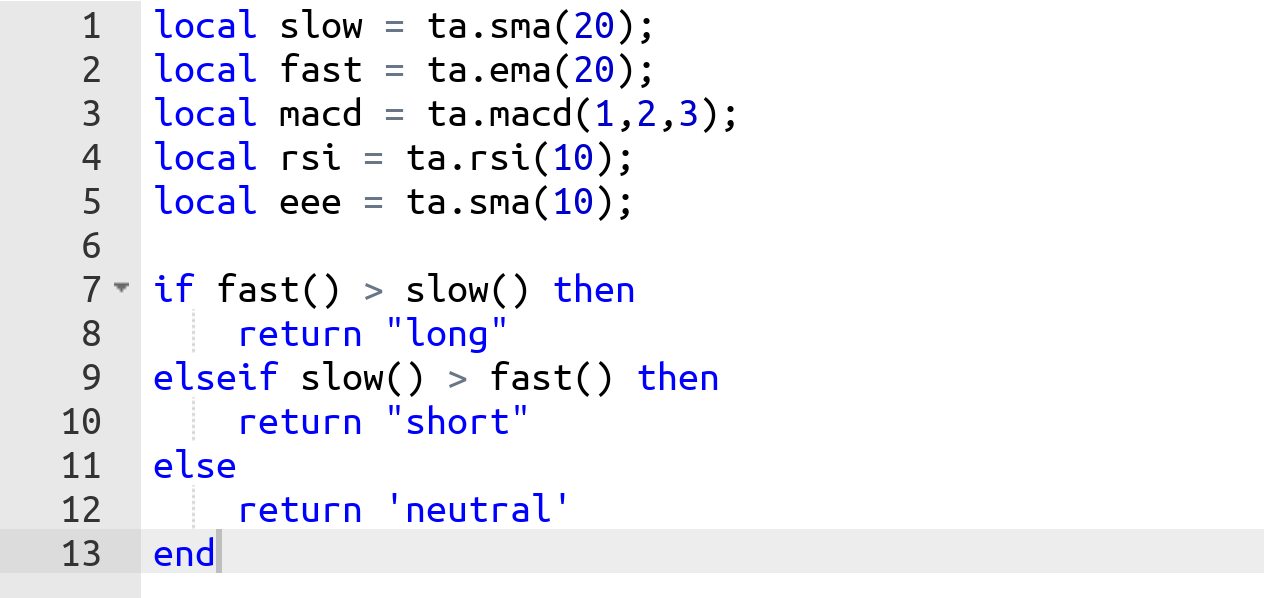
\includegraphics[height=0.3\textheight]{img/CIODE.png}
\end{figure}
}
\end{columns}
\end{frame}

\begin{frame}
    \frametitle{Návrh}
\begin{itemize}
    \item<2-> Distribuovaná architektúra
    \item<3-> Actor model
    \item<4-> Cloudové výpočetné prostredie
    \item<5-> Moderný implementačný jazyk
\end{itemize}
    \uncover<3->{
    \begin{figure}
        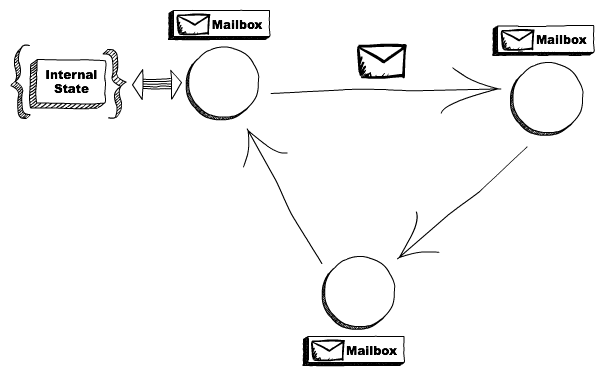
\includegraphics[height=0.5\textheight]{img/actors.png}
    \end{figure}
    }
\end{frame}

\begin{frame}
    \frametitle{Architektúra}
    \uncover<1->{
    \begin{figure}
        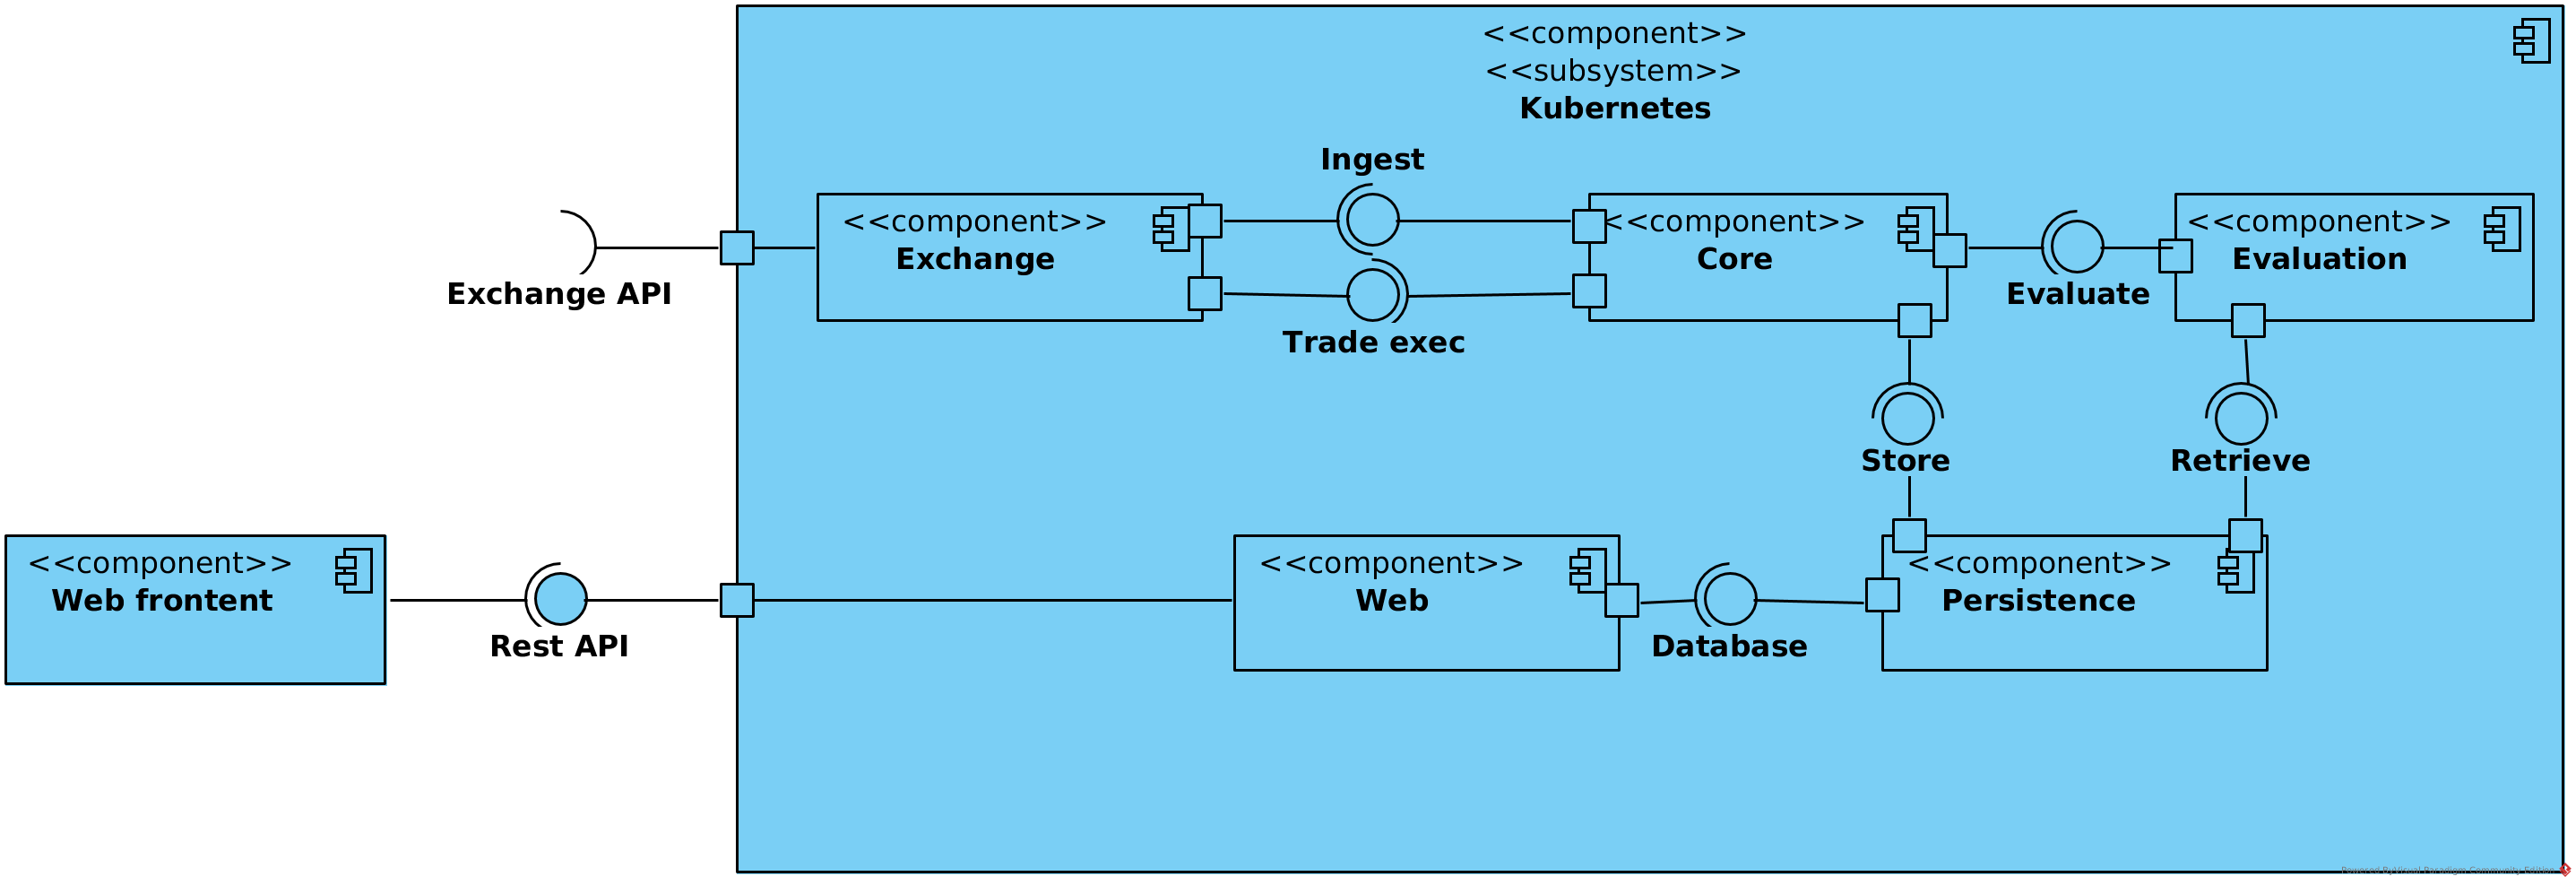
\includegraphics[width=0.9\textwidth]{img/comp.png}
    \end{figure}
    }
\begin{itemize}
    \item<1-> Systém rozdelený do komponentov
    \item<2-> Komponenty spravované systémom Kubernetes
    \begin{itemize}
        \item<2-> Monitoring a správa jednotlivých komponentov
        \item<2-> DNS pre service discovery
        \item<2-> Dynamické škálovanie na základe záťaže
    \end{itemize}
    \item<3-> Komunikácia pomocou ZeroMQ
    \item<4-> Jazyk Rust s knižnicou Actix
\end{itemize}
\end{frame}

% 7 000 LOC Rust
% 1500 JSX
% 340 verzií kontajnerov


\begin{frame}
    \frametitle{Výstupy práce}
    \begin{itemize}
        \item <1-> 2 Open source knižnice:
        \begin{itemize}
        \item <1-> Knižnica Actix-comm pre komunikáciu aktérov pomocou ZeroMQ
        \item <1-> Knižnica Actix-arch pre architekturálne komponenty
        \end{itemize}
        \item <2-> Systém dostupný na \textit{\href{http://trader.semtexzv.com}{trader.semtexzv.com}}
        \begin{itemize}
            \item <2-> Podporuje burzu Bitfinex
        \end{itemize}
    \end{itemize}
\end{frame}

\begin{frame}
    \frametitle{Meranie výkonu}
    Prístup :
    \begin{itemize}
        \item Virtuálny používatelia
        \item Zmena počtu použivateľov a konfigurácie systému
        \item Meranie latencie
    \end{itemize}

\uncover<2->{
    Primárny cieľ: latencia < 1s
    }
\end{frame}

\begin{frame}
    \frametitle{Namerané výsledky}
    \begin{figure}
        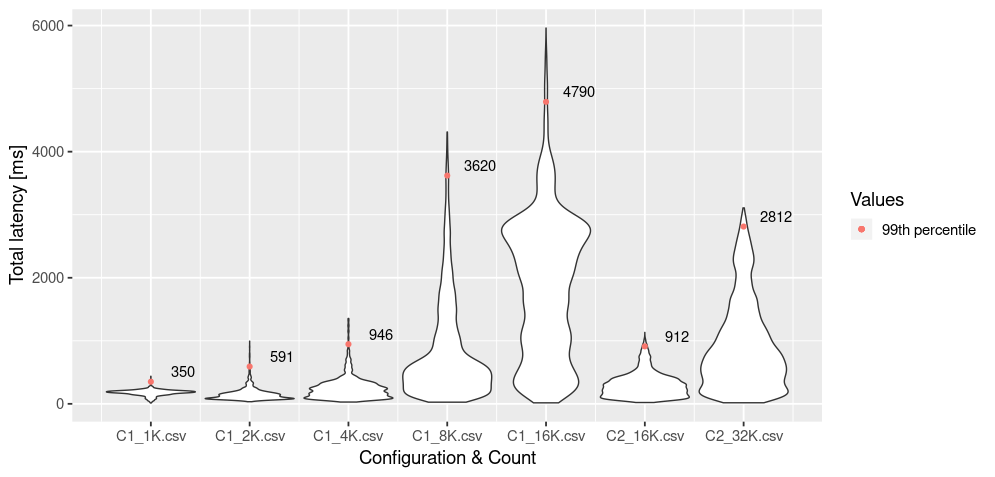
\includegraphics[width=\textwidth]{img/agg.png}
    \end{figure}
    \begin{itemize}
        \item<2-> Konfigurácia C1: \$ 30 - 4 000 priradení
        \item<3-> Konfigurácia C2: \$ 60 - 16 000 priradení
        \item<3-> Náročnejšie konfigurácie budú vyžadovať automatické škalovanie komponentov
    \end{itemize}

\end{frame}
\begin{frame}
    \frametitle{Budúcnosť}
    2 aspekty:
    \begin{enumerate}
        \item<2-> Samotný projekt
        \begin{itemize}
            \item <2-> Používateľské rozhranie
            \item <2-> Simulácia na historických dátach (Backtesting)
        \end{itemize}
        \item<3-> Architektúra
        \begin{itemize}
              \item <3-> Úprava knižníc actix-comm a actix-arch
              \item <3-> Použivanie pri dalších projektoch
        \end{itemize}
    \end{enumerate}
\end{frame}


% \bluepage{Ďakujem za pozornosť}

\begin{frame}
    \frametitle{Príklad stratégie}
    \begin{figure}
        \flushleft

        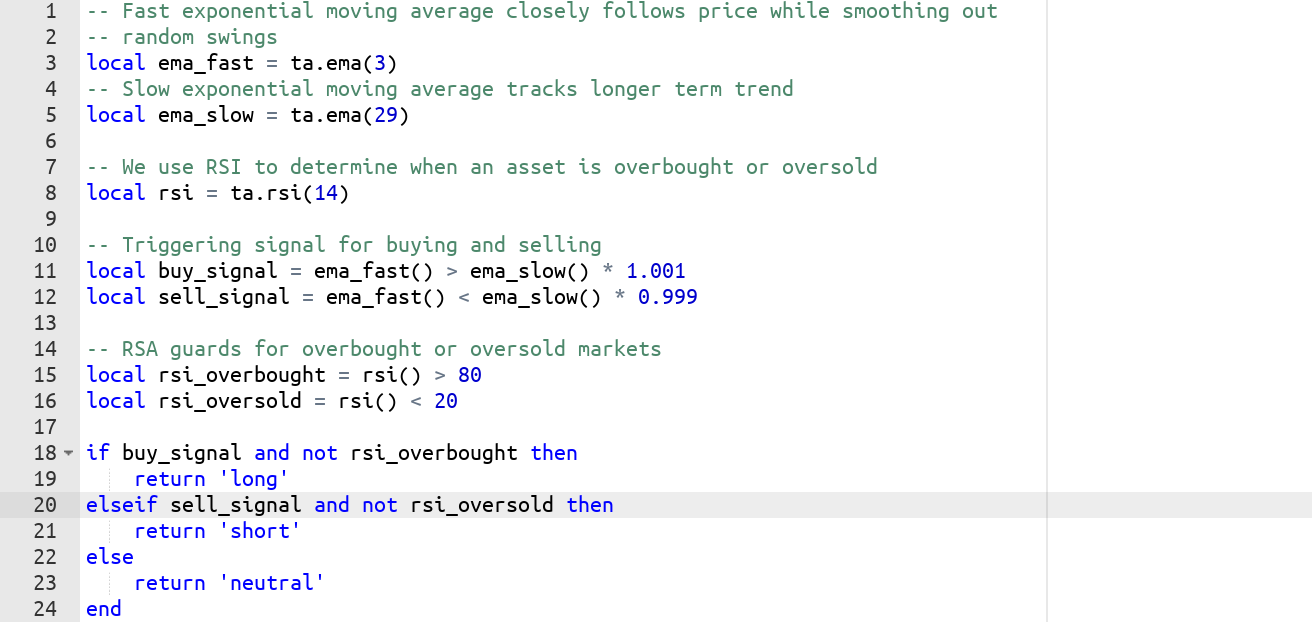
\includegraphics[width=0.95\textwidth]{img/strat.png}
    \end{figure}
    Strata 2\% po týždni používania
    \newline
    \begin{center}
    \uncover<2->{
        \textbf{Ďakujem za pozornosť}
    }

\end{center}
\end{frame}

\begin{frame}[noframenumbering]
    \frametitle{Otázky oponenta}
    \begin{enumerate}
        \item Prečo ste zvolili ZeroMQ ?
        \item Popíšte ako funguje Load balancing v komponente ktorý vyhodnocuje stratégie.
    \end{enumerate}
\end{frame}

\begin{frame}[noframenumbering]
    \frametitle{1. Voľba ZeroMQ}
    Možné alternatívy:
    \begin{enumerate}
        \item TCP
        \item ZeroMQ
        \item HTTP
    \end{enumerate}
    Výhody ZeroMQ:
    \begin{itemize}
        \item Komplexné topológie - Pub-sub
        \item Jednoduchý formát správ
        \item Nízka latencia
    \end{itemize}
\end{frame}

\begin{frame}[noframenumbering]
    \frametitle{Popis Distribúcie záťaže}
    \begin{columns}
        \column{0.5\textwidth}
        \begin{itemize}
            \item Nemožnosť použitia DNS distribúcie zátaže kvôli dlhodobým pripojeniam
            \item 1 distribučný kontajner, niekoľko výkonných
            \item Implementované ako sada aktérov v knižnici Actix-arch
            \item Distribúcia Round-robin na úrovni požiadavkov
        \end{itemize}
        \column{0.5\textwidth}
        \begin{figure}
            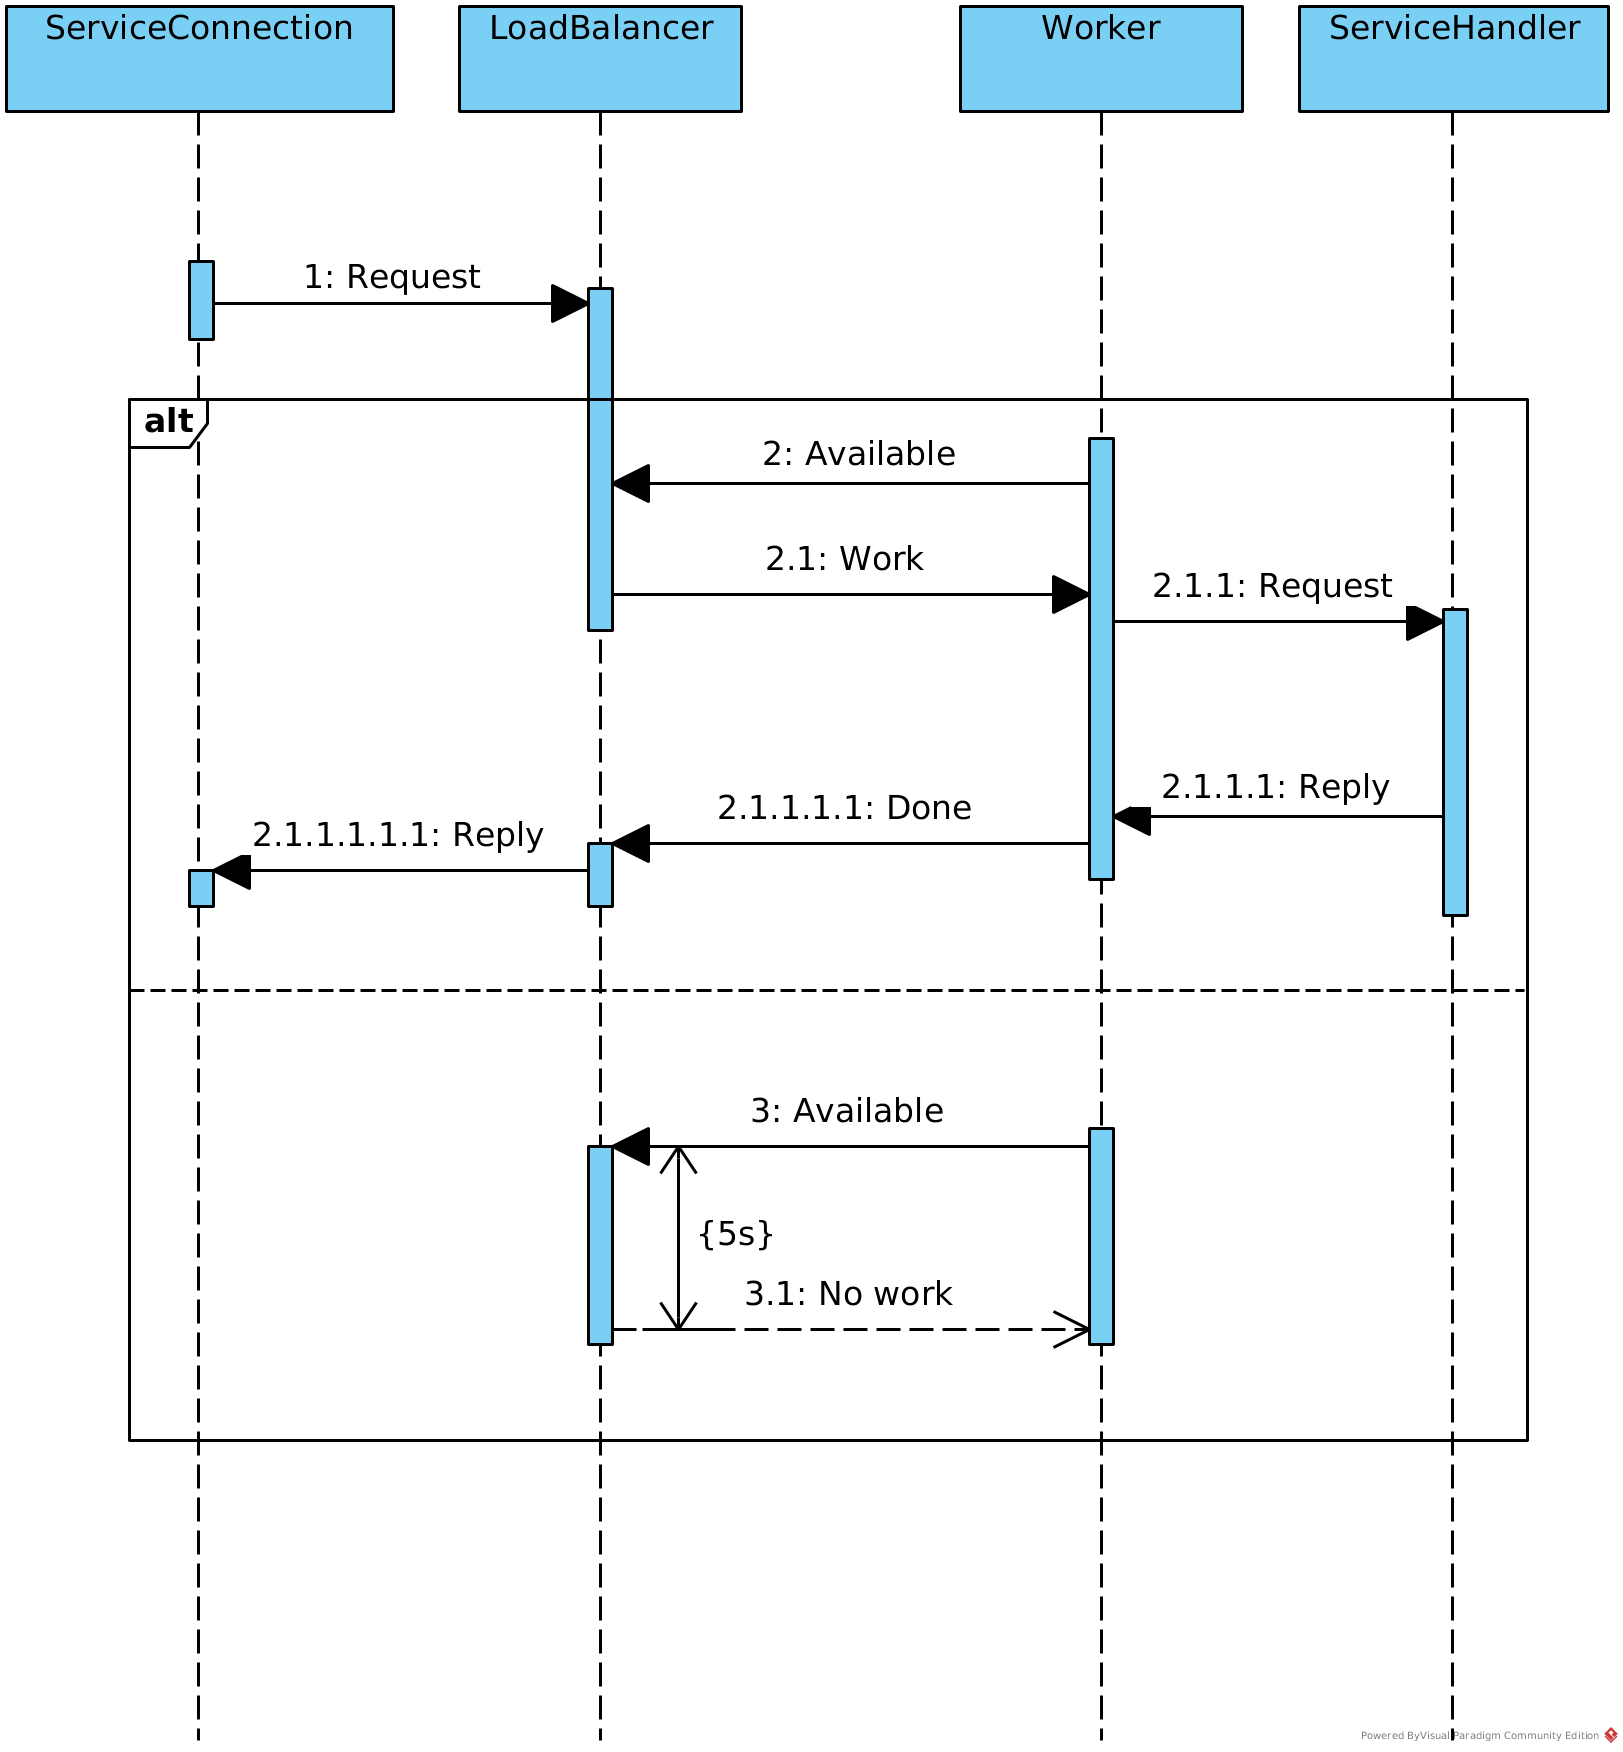
\includegraphics[height=0.65\textheight]{img/load_balancer.png}
        \end{figure}
    \end{columns}
\end{frame}



\end{document}
